\chapter{Аналитический раздел}\label{sec:analyth}

\section{Алгоритм волновой трассировки}

В своей работе Ли \cite{lee-orig} предлагал решать задачу о нахождении минимального пути в лабиринте путем представления пространства в виде матрицы. Каждая ячейка матрицы либо является препятствием, либо проходом. Рисунок \ref{fig:lee} демонстрирует принцип работы алгоритма. Здесь разными цветами отмечены ячейки с разными свойствами -- на рисунке \ref{fig:maze-init} белым цветом отмечена ячейка -- проход, черным -- препятствие. 

\begin{figure}[H]
	\captionsetup{singlelinecheck = false, justification=centering}
	\begin{subfigure}[b]{0.5\textwidth}
		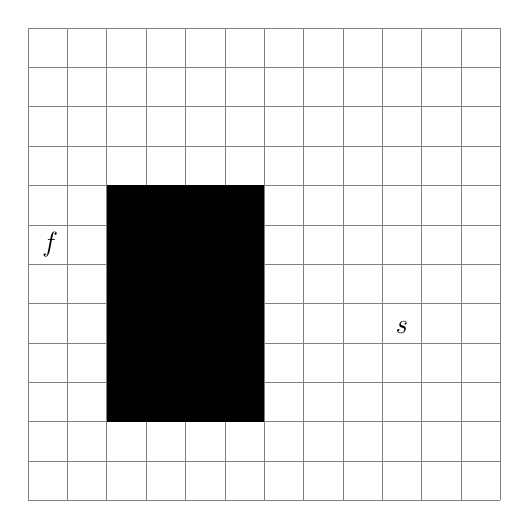
\begin{tikzpicture}
			\draw[step=0.5cm,gray,very thin] (0,0) grid (6,6);\\
			\fill[black] (1,1) rectangle (3,4);
			\draw (4.75,2.2) node{\textit{s}};
			\draw (0.3,3.25) node{\textit{f}};
%			\fill[pattern=north east lines] (0,0) rectangle (1,1);
		\end{tikzpicture}
	\caption{Начальная конфигурация}
	\label{fig:maze-init}

	\end{subfigure}
	\begin{subfigure}[b]{0.5\textwidth}
	\begin{tikzpicture}
		\draw[step=0.5cm,gray,very thin] (0,0) grid (6,6);\\
		\fill[black] (1,1) rectangle (3,4);
		\draw (4.75,2.2) node{\textit{s}};
		\draw (0.3,3.25) node{\textit{f}};
		\fill[pattern=north east lines] (4,2) rectangle (4.5,2.5);
		\fill[pattern=north east lines] (5,2) rectangle (5.5,2.5);
		\fill[pattern=north east lines] (4.5,2.5) rectangle (5,3);
		\fill[pattern=north east lines] (4.5,1.5) rectangle (5,2);
	\end{tikzpicture}
	\caption{Распространение волны}
	\label{fig:maze-wave}
\end{subfigure}
\caption{Матрица волнового алгоритма Ли}
\label{fig:lee}
\end{figure}


Начальная клетка осуществляет отправку сообщения четырем соседним. Сообщение представляет собой волну, продемонстрированную на рисунке \ref{fig:maze-wave}, Каждая захваченная волной ячейка, в свою очередь, отправляет сообщение четырем соседним. Сообщение представляет собой число, равное кратчайшему Манхэттенскому расстоянию от стартовой ячейки до ячейки -- получателя. 

Алгоритм имеет три стадии -- инициализация, распространение волны и восстановление пути, вторая стадия -- самая затратная с точки зрения вычислительных мощностей. Последняя стадия в рамках данной работы интереса не представляет, поэтому она будут опущена. 

\section{Поиск в ширину}

Одно из возможных решений алгоритма Ли основано на поиске в ширину\cite{bfs}. Существуют два варианта обхода графа при поиске в ширину: прямой обход графа («top-down») и обратный обход графа («bottom-up»). В рассматриваемом алгоритме используется прямой обход, который предполагает, что активные вершины помечают ближайшие соседние. В случае карты - лабиринта соседними вершинами являются верняя, нижняя, правая и левая ячейки карты, если они являются проходом, а не препятствием.
Алгоритм поиска в ширину реализуется с помощью очередей. Применяя его к задаче нахождения кратчайшего пути в лабиринте, можно сформировать следующее формальное описание:
\begin{enumerate}[label=(\roman*)]
	\setlength{\itemsep}{1.2pt}
	\setlength{\parskip}{0pt}
	\setlength{\parsep}{0pt}
	\item Создать пустую очередь;
	\item Поместить в очередь начальный узел, отметив его числом $0$;
	\item Извлечь из начала очереди ячейку $s$;\label{while}
	\item Если координаты ячейки $s$ совпадают с целевыми, то вернуть метку этой ячейки и завершить процедуру;
	\item Иначе, для каждой из четырех соседних клеток распространить волну (присвоить метку, большую метки рассматриваемой ячейки на 1);
	\item Если очередь пуста, то все ячейки были просмотрены, следовательно, целевая ячейка недостижима из начальной; завершить поиск.
	\item Вернуться к пункту \ref{while}.
\end{enumerate}


\section{Вывод}\label{sec:analyth-summ}
Реализация второго этапа алгоритма Ли (распространение волны) сводится к решению задачи поиска в ширину на графе, представленном в качестве карты обхода и её распараллеливанию. В целях упрощения задачи, этап восстановления пути будет опущен -- в качетсве результата достаточно предоставить найденное расстояние, иначе говоря, метку искомой вершины графа.
